%!TEX root = ../BoYu-Dissertation.tex
\graphicspath{{Figures/}}

\chapter{Architecture and Implementation} % (fold)
\label{cha:system_implementation}
To validate our computational approach, a prototype system EDAP (Event-driven awareness promotion) is implemented in this study. EDAP server provides a generic event-driven infrastructure for awareness promotion that can be applied in different application domain. EDAP client is a standalone Web-based interactive awareness system that is used to demonstrate the functionality of our approach. In this chapter, we first describe the architecture of the system. Then we describe the implementation details of the server and client.

\section{Architecture of EDAP} % (fold)
\label{sec:architecture_of_edap}
EDAP follows a typical client/server architecture model (Figure \ref{fig:edap_architecture}). The EDAP server provides the major functions of the event-driven awareness promotion, i.e. it maintains the knowledge representation, performs the knowledge updating and event processing. The EDAP client provides the visual and interactive environment that allows the user to perceive and interpret events,  generate new events, and manage subscriptions and visibility policies.

\begin{figure}[htbp] %  figure placement: here, top, bottom, or page
	\centering
	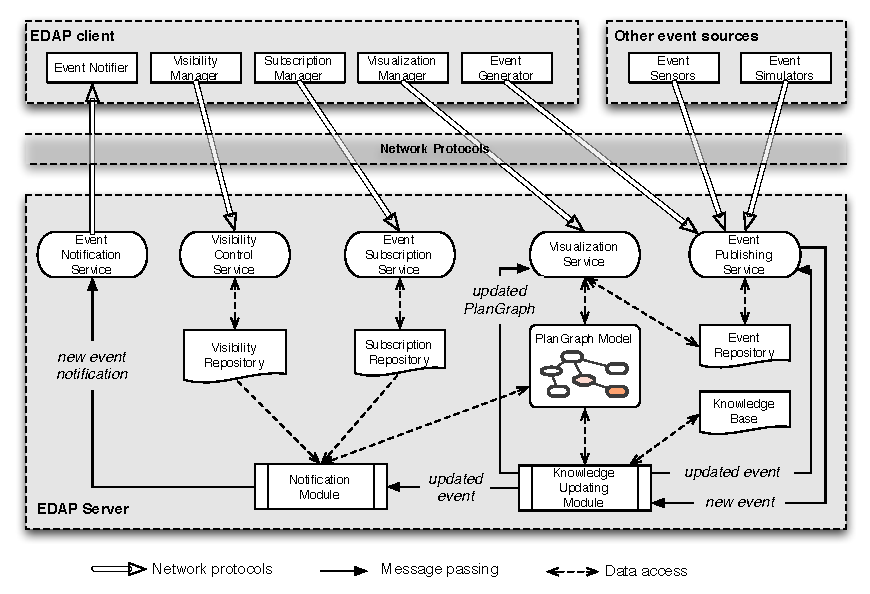
\includegraphics{edap_architecture.pdf} 
	\caption{Architecture of EDAP}
	\label{fig:edap_architecture}
\end{figure}

The interaction between the client and server follows the service-oriented network protocols. The REST protocol is used to implement the request/response communication style, i.e. clients initiate requests to servers and servers process requests and return appropriate responses. The COMET protocol is used to offer the push notification from the server to the client by maintaining a long-held HTTP request between them. 

The EDAP client provides several components that can interact with the server. The \emph{Event Generator} is used to create new events in the externalization process, and post the new events to the server for processing. The \emph{Visualization Manager} requests visualization specifications about the event view, activity view, and context view from the server, and render them in the client's interface. The \emph{Subscription Manager} requests the existing subscriptions from the server, provides the interface for the user to manage them or create new ones, and then send the modifications back to the server. The \emph{Visibility Manager} provides the similar function as the \emph{Subscription Manager} to manage visibility policies. The \emph{Event Notifier} establishes a long-polling connection with the server. Whenever a new event notification is sent from the server, it applies the corresponding notification style to notify the user. 

To respond to client requests, the EDAP server provides several components in the form of web services to handle the different types of requests. The \emph{Event Publishing Service} responds to the new events posted from the client or other event sources, stores them in the event repository, and notifies the \emph{Knowledge Updating Module} to process them. The \emph{Visualization Service} generates the visualization specifications for the event view and activity view based on the knowledge from PlanGraph model and event repository. The \emph{Event Subscription Service} responds to the \emph{Subscription Manager} and updates the subscription repository. The \emph{Visibility Control Service} responds to the \emph{Visibility Manager} and updates the visibility policy repository. The \emph{Event Notification Service} responds to the message passed from the \emph{Notification Module} whenever a new event notification is generated, and push it to the corresponding clients. Besides these service-oriented modules, the server also includes two important processing modules: the \emph{Knowledge Updating Module} perform the knowledge updating as described in Section \ref{sec:knowledge_updating_process} whenever new events are received; and the \emph{Notification Module} provides the local scope-based event notification mechanism (Section \ref{sec:event_notification_mechanism}) to distribute events. 

The communication between modules in the EDAP server is achieved through a limited form of the publish/subscribe interaction. Each module can publish important messages during its performance, and the other modules who need to respond to these messages need to subscribe to them. In this way, the interaction between modules can be asynchronous so that they do not block each other while waiting for others to finish their task. In addition, it provides a distributed interaction style that allows the different modules to be deployed across multiple machines. 
% section architecture_of_edap (end)

\section{Implementation of EDAP Server} % (fold)
\label{sec:implementation_of_edap_server}
The functional modules EDAP server is implemented using the Python programing language, and the web services are developed in the Django framework. The three data repositories, i.e. event, subscription and visibility repositories, as well as the knowledge base, are implemented as PostgreSQl databases. In the following, we describe the implementation details on major modules and the repositories are discussed within the respective modules that can manipulate them. 

\subsection{Service-oriented modules} % (fold)
\label{sub:service_oriented_modules}
The EDAP server includes five service-oriented modules to handle the different types of client requests. 

\paragraph*{Event Publishing Service} % (fold)
\label{par:event_publishing_service}
The \emph{Event Publishing Service} is the first responder to the new events that are published to the system, and its major responsibility is to store the events in the event repository. There are two types of event sources where the \emph{Event Publishing Service} can receive events:

\begin{enumerate}
	\item Events can come externally from the different types of clients as HTTP requests, including the EDAP client or other event sensors or simulators. For these events, after storing them in the repository, the service also needs to send out a \emph{`NewEvent'} message notifying the \emph{Knowledge Updating Module} to perform knowledge updating on the new event.
	\item They can also come from the \emph{Knowledge Updating Module} as it generates new derived or anticipatory events. These events are published by the \emph{Knowledge Updating Module} as \emph{`UpdatedEvent'} messages, and the \emph{Event Publishing Service} needs to subscribe to them and store them in the repository. 
\end{enumerate}

The events received by the \emph{Event Publishing Service} are described as attribute-value tuples, and the service needs to store these events in the event repository. The event repository needs to be semi-structured as the different event types supported by the system can have different set of attributes. However, this cannot be directly achieved in a relational database like PostgreSQl. As a result, we only store the header of each event directly in the data tables, but add two additional long text field (\emph{payload} and \emph{opencontent}) for each record. These two fields store the XML formatted tuples corresponding to the attributes in the event's payload and open content. Besides the event table that stores all the events, the event repository also includes a relation table to record the event chains or event propagation trees. Whenever an event is added to the repository, a new record is added to the event development table as well with the id of parent event (null for original events) and the current event, along with the label indicating the type of the event. Figure \ref{fig:event_repository} shows the data tables in the event repository. 

\begin{figure}[htbp] %  figure placement: here, top, bottom, or page
	\centering
	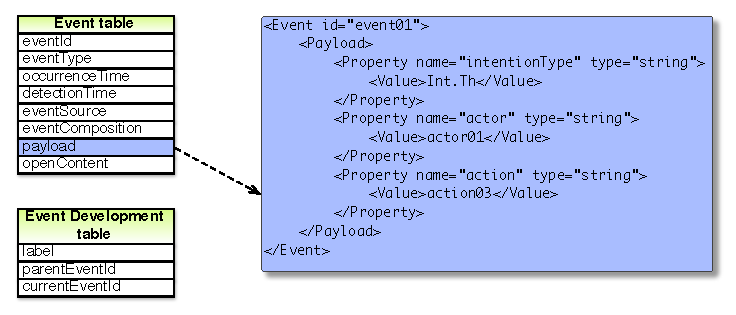
\includegraphics{event_repository.pdf} 
	\caption{Data tables in the event repository}
	\label{fig:event_repository}
\end{figure}
% paragraph event_publishing_service (end)

\paragraph*{Visualization Service} % (fold)
\label{par:visualization_service}
The \emph{Visualization Service} responds to the client's request for visualizing the event view or activity view. The service retrieves the necessary data from event repository or PlanGraph model, uses it to generate a visualization specification in the JSON format and sends it back to the client. 

For the request to visualize the event view given the current event under interpretation, the service searches the event repository recursively to find all the events that are included in the event propagation tree, and generates a JSON object to represent the tree structure.

In order to generate the visualization specification for the activity view, the service maintains the most recent version of the local scopes and dependency network constructed from the PlanGraph model. The \emph{Visualization Service} subscribes to the message \emph{`updatedPlanGraph'} that is published by the \emph{Knowledge Updating Module} each time the PlanGraph model is changed. Hence, whenever the \emph{Visualization Service} receives such message, it uses the PlanGraph model to reconstruct the local scopes and dependency network so that it always keeps the newest version. Whenever the client requests an activity view given a specific user, the user's local scope is first retrieved, and the entities in the local scope are added to the visualization specification. Then the entities in the local scope are searched in the dependency network recursively to find all the other entities that have dependency relations with them, and these entities outside the local scope are added to visualization specification.
% paragraph visualization_service (end)

\paragraph*{Event Subscription Service} % (fold)
\label{par:event_subscription_service}
The \emph{Event Subscription Service} responds to the client's request to list all the current subscriptions, add a new subscription, modify or delete an existing subscription. The existing subscription of each user is stored in the subscription repository. If the request is to add a new subscription, a new record will be added into the repository. If the request is to modify or delete an existing one, the subscription id will be used to identify the record in the repository and perform the update or delete operation. 

Because the event pattern in each subscription is semi-structured with multiple filter expressions, we also use the XML formatted text field to store the filters for each subscription. Figure \ref{fig:sub_repository} shows the subscription table with an example of the XML formatted event pattern that include all the three types of filter expressions discussed in Section \ref{sub:managing_subscriptions}.

\begin{figure}[htbp] %  figure placement: here, top, bottom, or page
	\centering
	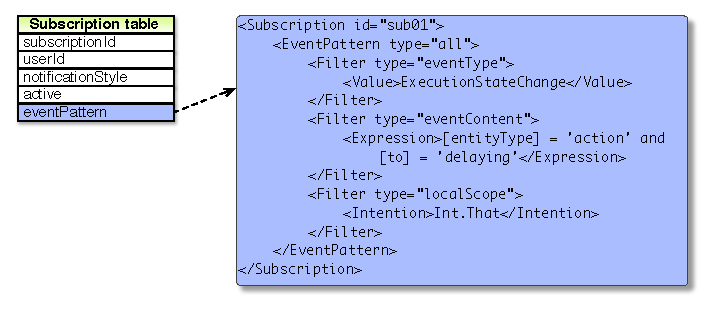
\includegraphics{sub_repository.pdf} 
	\caption{An example subscription record}
	\label{fig:sub_repository}
\end{figure}
% paragraph event_subscription_service (end)

\paragraph*{Visibility Control Service} % (fold)
\label{par:visibility_control_service}
The \emph{Visibility Control Service} works in the similar way as the \emph{Event Subscription Service}, to manipulate the visibility repository to retrieve, add, modify or delete visibility policies. Unlike the subscriptions, each visibility policy has three semi-structured fields: the \emph{eventPattern} is similar to the event pattern in subscriptions, the \emph{receiverPattern} includes the filter expressions that are used to define the receivers to whom the event is visible, and \emph{attributeList} is the list of visible attributes. Figure \ref{fig:vis_repository} shows an example of a record in the visibility repository.
\begin{figure}[htbp] %  figure placement: here, top, bottom, or page
	\centering
	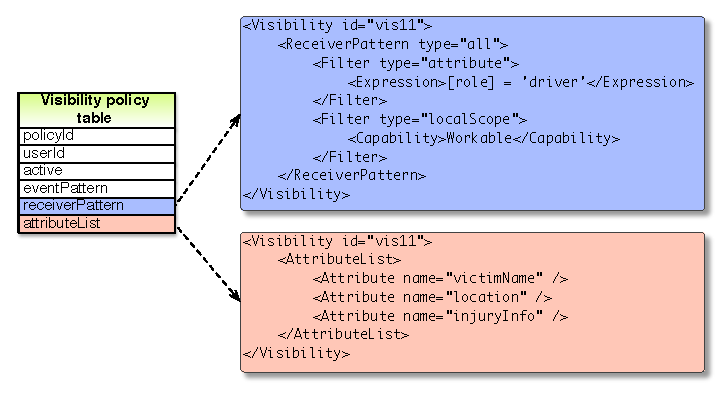
\includegraphics{vis_repository.pdf} 
	\caption{An example visibility policy record}
	\label{fig:vis_repository}
\end{figure}
% paragraph visibility_control_service (end)

\paragraph*{Event Notification Service} % (fold)
\label{par:event_notification_service}
The \emph{Event Notification Service} maintains a long polling connection with each client so that it can push new event notifications to the client. The service stores a routing table that maps each user id to the corresponding client connection. The service subscribes to the message \emph{`newEventNotification'} that is published by the \emph{Notification Module} each time a new event notification is generated. Whenever the \emph{Event Notification Service} receives such a message, it searches the routing table to find a match between the receiver of the notification and the client connection. If a connection is found, the service pushes the event notification to the corresponding user via the client connection. 
% paragraph event_notification_service (end)
% subsection service_oriented_modules (end)

\subsection{The Knowledge updating module} % (fold)
\label{sub:the_knowledge_updating_module}
The \emph{Knowledge Updating Module} performs the knowledge updating process as we described in Section \ref{sec:knowledge_updating_process}. As the \emph{Knowledge Updating Module} manipulates the PlanGraph model, we first describe how the PlanGraph model is implemented, then discuss the implementation of the knowledge updating process.

\paragraph*{Implementation of the PlanGraph} % (fold)
\label{par:implementation_of_the_plangraph}
The PlanGraph is implemented in the object-oriented paradigm as a dynamic data structure by several data objects. The overall \emph{PlanGraph} object points to the root plan node. Each \emph{PlanNode} objects includes attributes recording the parent node and the subsidiary plan nodes, which together allows the recursive traverse throughout the PlanGraph hierarchy. 

The \emph{PlanNode} has three types of subsidiary classes, corresponding to the three types of nodes in the PlanGraph model.

\begin{enumerate}
	\item Each \emph{ActionNode} defines the properties of an action, such as the type of the action, whether it is a basic or complex action, the execution state, the current recipe of the action. Each \emph{ActionNode} also includes two slots to store the actors' intentions and capabilities towards the action. Besides, each \emph{ActionNode} includes a list of parameters and the conditions.
	\item Each \emph{ParamNode} object represents a parameter that includes the type of the parameter, the execution state, the values, and the list of conditions about the parameter.
	\item Each \emph{CondNode} object represents a condition that includes the type of the parameter, the execution state, and an expression indicating the content of the condition.
\end{enumerate}
\begin{figure}[htbp] %  figure placement: here, top, bottom, or page
	\centering
	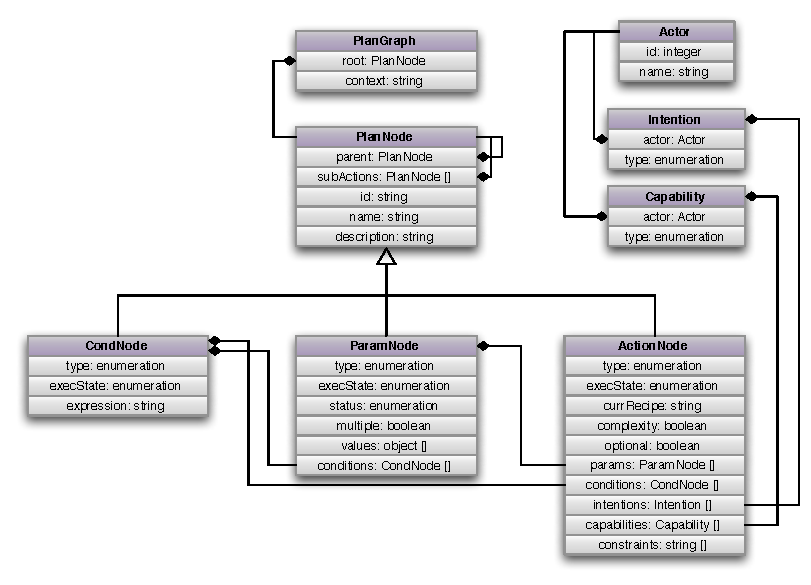
\includegraphics{pg_class_diagram.pdf} 
	\caption{The class diagram of the PlanGraph}
	\label{fig:pg_class_diagram}
\end{figure}
% paragraph implementation_of_the_plangraph (end)

\paragraph*{Implementation of the knowledge updating process} % (fold)
\label{par:implementation_of_the_knowledge_updating_process}
The \emph{Knowledge Updating Module} includes four subsidiary modules, complying with the four steps of the knowledge updating process. 

\begin{enumerate}
	\item \emph{Association} sub-module establishes the association between the input event and the current PlanGraph mode by searching all the nodes in the PlanGraph. It starts with the recognition of event type for each input event, as the different event types are treated differently. The association is implemented as a native function in Python that follows the search strategies we discussed in Section \ref{sub:association}. Once an association is found, it updates the value of the corresponding node in the PlanGraph, and then add the pointer to the node into the event object.
	\item \emph{Assessment} sub-module evaluates each event check how it can lead to changes towards the action performance, such as the execution state change of an action, or a condition. This sub-module is achieved by defining a set of assessment rules and employing a knowledge engine Pyke to enable the forward chaining inference. The knowledge engine uses the PlanGraph to assess all the possible changes due to the new information stored in the event, and then generate new events to represent these changes. Whenever a new event is generated in this step, the module publishes a new \emph{`NewEvent'} message, so that the other modules who subscribe to it can get notified.
	\item \emph{Elaboration} sub-module advances the collaborative activity from the system side based on the change from the new event. The elaboration is achieved with the support of two types of knowledge stored in the knowledge base: (1) the recipe knowledge about how to derive an action into a sequence of parameters, pre-conditions, and subsidiary actions, how to identify a unbound parameter, or how to satisfy a condition, etc.; (2) the knowledge about actor roles and the potential intentions and capabilities towards actions. These two types of knowledge are stored in the \emph{knowledge base} in the form of a PostgreSQl database. The content of each recipe is stored in an XML formatted text field along with other general information about the recipe. The actor role specifications are stored in a data table mapping each role to the potential intended action type, or the actions that the actors in the role are capable of performing.
	\fxwarning{add an example recipe here.}
	\item \emph{Propagation} sub-module is a standard Bayesian network-based reasoning process. This module first constructs the dependency network from the PlanGraph model following the algorithm described in Section \ref{sub:representing_dependencies}. Then we employ the open source Python library, OpenBayes, to propagate the state change in the dependency network. Based on the results of the propagation, we generate new events to represent these changes, and new \emph{`NewEvent'} messages will be published to notify other modules.
\end{enumerate}

After the four steps have been performed, the knowledge updating module publishes two new messages \emph{`UpdatedEvent'} and \emph{`UpdatedPlanGraph'}. The former is used by the \emph{Notification Module} to start generating event notifications, and the latter notifies the \emph{Visualization Service} to reconstruct the local scopes and dependency network.
% paragraph implementation_of_the_knowledge_updating_process (end)
% subsection the_knowledge_updating_module (end)

\subsection{The Notification module} % (fold)
\label{sub:the_notification_module}
The \emph{Notification Module} performs the event notification algorithms to generate event notifications after the knowledge updating process is done on each event, i.e. whenever it receives a new message \emph{`UpdatedEvent'} from the \emph{Knowledge Updating Module}. The \emph{Notification Module} generates event notifications in three steps, and different type of knowledge is used in each step.

\begin{enumerate}
	\item The PlanGraph is used in the first step to perform the local scope-based filtering as described in Section \ref{sub:event_filtering_algorithm}. The module implements the $FILTER\textrm{-}LS$ algorithm as a standard Python function and execute it on each user participated in the PlanGraph. If the function returns true, the second step is performed.
	\item During the second step, the user's subscriptions are retrieved from the subscription repository, and the event is evaluated against each of the subscriptions. If the event matches the event pattern of a subscription, the third step is performed.
	\item In this step, the user's visibility policies are retrieved from the visibility repository, and the $APPLY\textrm{-}VIS$ algorithm (Section \ref{sub:controlling_visibility}) is implemented to apply the visibility policies to the event notification. If function returns true, i.e. the event is visible to the actor, then the corresponding event notification is generated.
\end{enumerate}

Once an event notification is generated, the \emph{Notification Module} publishes a new messages \emph{`NewEventNotification'}, which is subscribed by the \emph{Event Notification Service} who will push the event notification to the user's client.
% subsection the_notification_module (end)
% section implementation_of_edap_server (end)

\section{Implementation of EDAP Client} % (fold)
\label{sec:implementation_of_edap_client}
The EDAP client is a Web-based client provides the user with the lightweight HTML + JavaScript user interface to the awareness system. The EDAP client is implemented by using several Open Source JavaScript libraries: JQuery framework for the interface layout, the OpenLayers mapping library to provide the geographic context view, and the d3 library to generate the event view and activity view. The thin client design allows the user to easily access the system without installing any software or plug-ins. 

The EDAP client is developed for supporting awareness in the motivating scenario of emergency response described in Section \ref{sub:geo_collaboration}. Within this scenario, the awareness process can involve multiple actors. Imagine the occurrence of an unexpected event indicating a traffic jam that blocks the route for delivering a victim to a decontamination station. This event is first perceived by the transportation manager, who interprets the event as the cause of a delay for a vehicle that is used to deliver a victim to the decontamination station as scheduled. As a result, the decontamination manager’s intention to have the victim delivered at the decontamination station on time becomes problematic, which is further interpreted as a cause for delay on the decontamination operation. Furthermore, the delay on decontamination could impact the victim manager due to the temporal dependency between decontamination and medical treatment. The victim manager may have to re-schedule the victim so that the medical resource could be assigned to another victim.

Figure \ref{fig:main_interface} shows the main interface of the EDAP client from the victim manager’s perspective. We provide three inter-linked visual representations. 

\begin{figure}[htbp] %  figure placement: here, top, bottom, or page
	\centering
	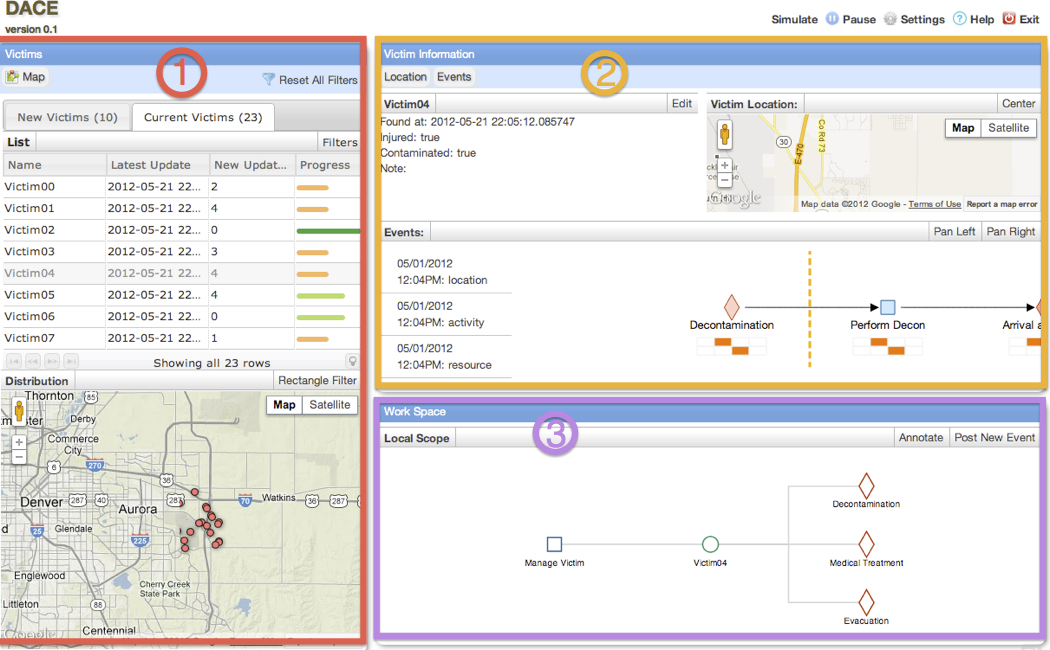
\includegraphics[width=5.5in]{main_interface.jpg} 
	\caption{The main interface of the EDAP client}
	\label{fig:main_interface}
\end{figure}


\begin{enumerate}
	\item The \emph{event view} provides a list of current events notified to the victim manager. The victim manager can click on each event to activate the event propagation tree to backtrack the event development.
	\item The \emph{activity view} shows the goals, activities, resources assigned to the current victim, which forms the local scope of the victim manager, where he/she can interpret the event and project state changes based on established understanding of the situation.
	\item The \emph{context view} consists of interactive data visualization tools to explore the contextual information. For the victim manager, the interface allows him/her to monitor the status of every victim that has been reported. A dynamic query interface is used for filtering the victims based on attributes, time, and geographical locations.
\end{enumerate}

\fxwarning{use the scenario to run through the whole process to demonstrate the functionalities: from notification, to event view, to activity view, to the generate new events, to manage subscription, to manage visibility. }
% section implementation_of_edap_client (end)
% chapter system_implementation (end)




 

